% نمایش برداری دو آرایش از توزیع‌های سه‌برچسبی
% مراکز در دو پنل ثابت‌اند؛ تنها موقعیت نمونه‌های طبقه اول تفاوت دارد.
% تصویر توضیحی است؛ اعداد و نسبت‌های شکل نتیجه آزمایش نیستند.
\begingroup
\definecolor{marginedge}{HTML}{61748C}
\definecolor{marginpurple}{HTML}{EEEAFB}
\definecolor{marginorange}{HTML}{FFF0E6}
\definecolor{margingreen}{HTML}{DFF4EE}
\definecolor{marginblue}{HTML}{26829A}
\definecolor{marginred}{HTML}{D16C69}
\definecolor{marginviolet}{HTML}{8168BC}
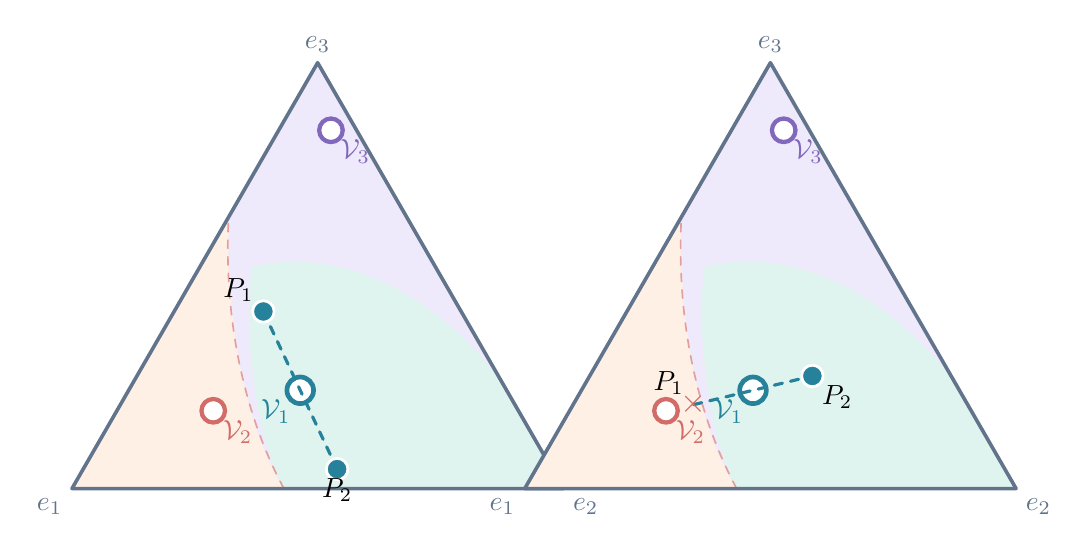
\begin{tikzpicture}[x=1.30cm,y=1.30cm,line cap=round,line join=round]
% پنل چپ: مراکز ثابت، دو نمونه با پراکندگی بیشتر و تصمیم صحیح.
\begin{scope}
  \begin{scope}
    \clip (0,0)--(4.8,0)--(2.4,4.16)--cycle;
    \fill[marginpurple] (0,0) rectangle (4.8,4.16);
    \fill[marginorange] (0,0)--(1.53,2.65)
        .. controls (1.50,1.70) and (1.68,0.60) .. (2.07,0)--cycle;
    \fill[margingreen] (2.07,0)
        .. controls (1.78,0.50) and (1.67,1.66) .. (1.76,2.17)
        .. controls (2.80,2.41) and (4.04,1.73) .. (4.80,0)--cycle;
    \draw[marginred!65,dashed,line width=.6pt] (2.07,0)
       .. controls (1.68,.73) and (1.48,1.65) .. (1.53,2.65);
  \end{scope}
  \draw[marginedge,line width=1.3pt] (0,0)--(4.8,0)--(2.4,4.16)--cycle;
  \node[below left, text=marginedge] at (0,0) {$e_1$};
  \node[below right, text=marginedge] at (4.8,0) {$e_2$};
  \node[above, text=marginedge] at (2.4,4.16) {$e_3$};
  % مراکز طبقات
  \draw[marginred,line width=1.55pt,fill=white] (1.38,.76) circle (.115);
  \node[below right, text=marginred] at (1.38,.76) {$\mathcal V_2$};
  \draw[marginviolet,line width=1.55pt,fill=white] (2.53,3.50) circle (.115);
  \node[below right, text=marginviolet] at (2.53,3.50) {$\mathcal V_3$};
  \draw[marginblue,line width=1.7pt,fill=white] (2.23,.96) circle (.13);
  \node[below left,text=marginblue] at (2.23,.96) {$\mathcal V_1$};
  % دو نمونه طبقه اول با مرکز میانگین V1
  \draw[marginblue,dashed,line width=1.15pt] (1.87,1.73)--(2.23,.96)--(2.59,.19);
  \filldraw[draw=white,fill=marginblue,line width=1pt] (1.87,1.73) circle (.105);
  \node[above left] at (1.87,1.73) {$P_1$};
  \filldraw[draw=white,fill=marginblue,line width=1pt] (2.59,.19) circle (.105);
  \node[below] at (2.59,.19) {$P_2$};
\end{scope}
% پنل راست: مراکز دقیقاً همان‌اند، فاصله نمونه‌ها از مرکز کمتر است،
% اما نمونه اول به ناحیه تصمیم طبقه دوم منتقل می‌شود.
\begin{scope}[xshift=5.75cm]
  \begin{scope}
    \clip (0,0)--(4.8,0)--(2.4,4.16)--cycle;
    \fill[marginpurple] (0,0) rectangle (4.8,4.16);
    \fill[marginorange] (0,0)--(1.53,2.65)
        .. controls (1.50,1.70) and (1.68,0.60) .. (2.07,0)--cycle;
    \fill[margingreen] (2.07,0)
        .. controls (1.78,0.50) and (1.67,1.66) .. (1.76,2.17)
        .. controls (2.80,2.41) and (4.04,1.73) .. (4.80,0)--cycle;
    \draw[marginred!65,dashed,line width=.6pt] (2.07,0)
       .. controls (1.68,.73) and (1.48,1.65) .. (1.53,2.65);
  \end{scope}
  \draw[marginedge,line width=1.3pt] (0,0)--(4.8,0)--(2.4,4.16)--cycle;
  \node[below left, text=marginedge] at (0,0) {$e_1$};
  \node[below right, text=marginedge] at (4.8,0) {$e_2$};
  \node[above, text=marginedge] at (2.4,4.16) {$e_3$};
  \draw[marginred,line width=1.55pt,fill=white] (1.38,.76) circle (.115);
  \node[below right, text=marginred] at (1.38,.76) {$\mathcal V_2$};
  \draw[marginviolet,line width=1.55pt,fill=white] (2.53,3.50) circle (.115);
  \node[below right, text=marginviolet] at (2.53,3.50) {$\mathcal V_3$};
  \draw[marginblue,line width=1.7pt,fill=white] (2.23,.96) circle (.13);
  \node[below left,text=marginblue] at (2.23,.96) {$\mathcal V_1$};
  \draw[marginblue,dashed,line width=1.15pt] (1.65,.82)--(2.23,.96)--(2.81,1.10);
  % نمونه سمت چپ متعلق به طبقه اول است، اما در ناحیه رقیب قرار دارد.
  \node[marginred,font=\bfseries\large] at (1.65,.82) {$\times$};
  \node[above left] at (1.65,.82) {$P_1$};
  \filldraw[draw=white,fill=marginblue,line width=1pt] (2.81,1.10) circle (.105);
  \node[below right] at (2.81,1.10) {$P_2$};
\end{scope}
\end{tikzpicture}
\endgroup
